% a standalone tikz figure
\documentclass{article}
\usepackage{tikz}
\usetikzlibrary{matrix}

\begin{document}
% \begin{tikzpicture}
% \draw (0,0) -- (1,0) -- (1,1) -- (0,1) -- cycle;
% \draw (0.5,0.5) node {Hello};
% \draw (0.5,0.5) node {Hello};
% \end{tikzpicture}

% \begin{tikzpicture}
%     \draw (-1.5,0) -- (1.5,0);
%     \draw (0,-1.5) -- (0,1.5);
%     \draw (0,0) circle [radius=1cm];
%     \draw[step=.5cm] (-1.4,-1.4) grid (1.4,1.4);
%   \end{tikzpicture}

%   \begin{tikzpicture}
%     % draw help lines
%     \draw[help lines] (0, 0) grid (8, 8);
%     \draw (3, 3) circle [radius=1cm];

%     \node [matrix,draw=black,anchor=base,every node/.style={draw=red}] (m) at (3, 3) {
%         \node{the quick}; & \node{rown}; \\
%     };

%   \end{tikzpicture}

  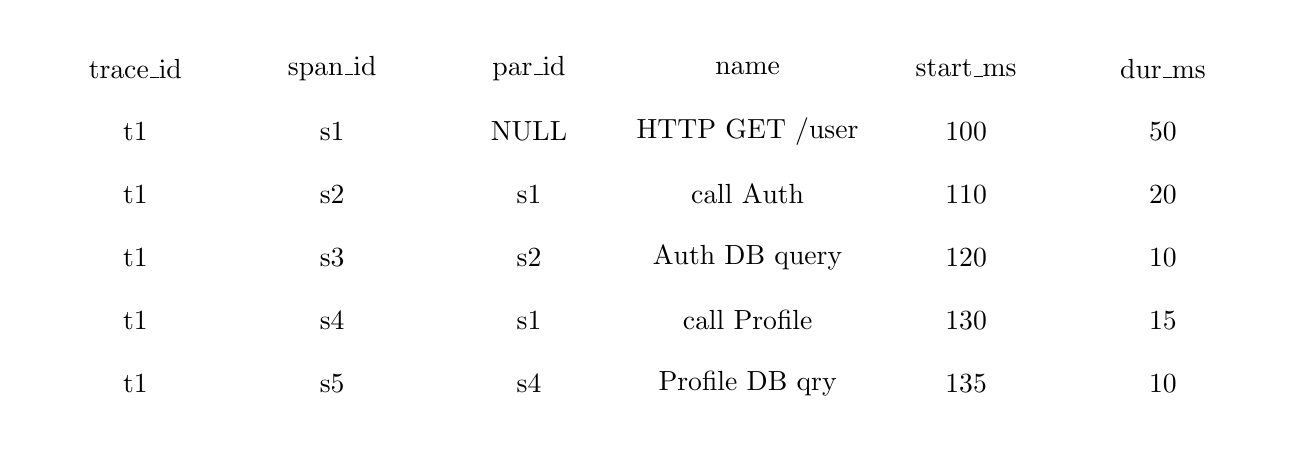
\begin{tikzpicture}
    \matrix[matrix of nodes,
            nodes={minimum width=2.5cm, minimum height=0.8cm, anchor=center}
    ] (m) {
      trace\_id & span\_id & par\_id & name & start\_ms & dur\_ms \\
      t1 & s1 & NULL & HTTP GET /user   & 100 & 50 \\
      t1 & s2 & s1   & call Auth         & 110 & 20 \\
      t1 & s3 & s2   & Auth DB query     & 120 & 10 \\
      t1 & s4 & s1   & call Profile      & 130 & 15 \\
      t1 & s5 & s4   & Profile DB qry    & 135 & 10 \\
    };
  \end{tikzpicture}

  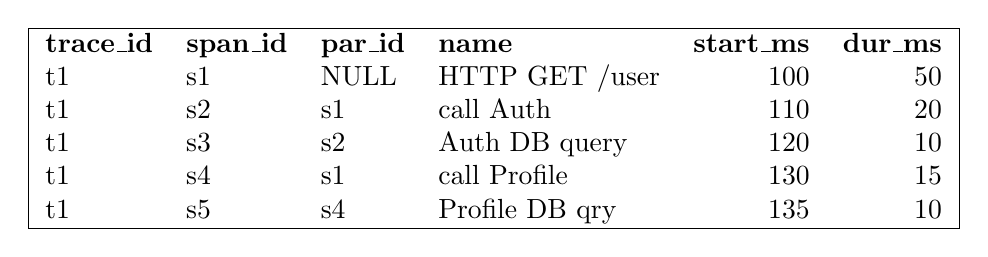
\begin{tikzpicture}
    \node[inner sep=0] (T) {%
      \begin{tabular}{l l l l r r}
      \textbf{trace\_id} & \textbf{span\_id} & \textbf{par\_id} & \textbf{name} & \textbf{start\_ms} & \textbf{dur\_ms}\\
      t1 & s1 & NULL & HTTP GET /user & 100 & 50 \\
      t1 & s2 & s1   & call Auth       & 110 & 20 \\
      t1 & s3 & s2   & Auth DB query   & 120 & 10 \\
      t1 & s4 & s1   & call Profile    & 130 & 15 \\
      t1 & s5 & s4   & Profile DB qry  & 135 & 10 \\
      \end{tabular}%
    };
    \draw (T.north west) rectangle (T.south east); % optional border
    \end{tikzpicture}
\end{document}